% LaTeX support: latex@mdpi.com
% Template source: MDPI ACS LaTeX template package, downloaded 2026-05-20.

\documentclass[jmse,article,submit,pdftex,oneauthor]{Definitions/mdpi}

\firstpage{1}
\makeatletter
\setcounter{page}{\@firstpage}
\makeatother
\pubvolume{1}
\issuenum{1}
\articlenumber{0}
\pubyear{2026}
\copyrightyear{2026}
\datereceived{ }
\daterevised{ }
\dateaccepted{ }
\datepublished{ }
\setlength{\headheight}{20pt}

\Title{MRV-EffScreen: Temporal Generalization and Consistency Screening of Ship Energy-Efficiency Labels from Public THETIS-MRV Emission Reports}

\newcommand{\orcidauthorA}{0009-0002-0772-5138}

\Author{Bo Li $^{1}$\orcidA{}}
\AuthorNames{Bo Li}

\address{%
$^{1}$ \quad China Maritime Service Center, Beijing, China; li.bo@cmaritime.com.cn}

\corres{Correspondence: li.bo@cmaritime.com.cn}

\abstract{Public ship-level emission reports provide a transparent basis for data-driven maritime decarbonization studies, but predictive analyses must avoid target leakage and must be evaluated under realistic temporal shifts. This study proposes MRV-EffScreen, a reproducible framework for relative ship energy-efficiency stratification and emission consistency screening using public EU THETIS-MRV emission reports. We harmonized 2018--2024 public records, constructed ship-type-year tertile labels from CO2 emissions per distance, and evaluated non-leakage static and non-emission operational features under a temporal design. The processed dataset contained 90,745 records, 22,551 unique IMO numbers, and 17 ship types; the main labeled 2018--2023 experiment contained 73,045 records. Histogram-based gradient boosting with non-emission operational features achieved Macro-F1 = 0.603 and balanced accuracy = 0.605 on the 2023 temporal test set, while the best random stratified split reached Macro-F1 = 0.657. Ship-type-specific models improved some categories but were not uniformly superior. A separate consistency-screening module combining Isolation Forest, Local Outlier Factor, and regression residual ranking identified 226 all-method candidates at a 2\% threshold. These candidates are intended for manual inspection, not compliance adjudication.}

\keyword{green shipping; THETIS-MRV; ship energy efficiency; temporal generalization; machine learning; anomaly screening; emission consistency; maritime decarbonization}

\begin{document}

\section{Introduction}

International shipping is central to global trade and remains a difficult-to-decarbonize transport sector. The Fourth IMO Greenhouse Gas Study reported that greenhouse gas emissions from shipping increased between 2012 and 2018 and that shipping accounted for a measurable share of global anthropogenic emissions \cite{imo_fourth_ghg_study_2020}. The 2023 IMO greenhouse gas strategy further strengthened the long-term ambition for international shipping to reach net-zero greenhouse gas emissions by or around 2050, with indicative checkpoints for 2030 and 2040 \cite{imo_2023_ghg_strategy}. Operational instruments such as the Energy Efficiency Existing Ship Index (EEXI) and Carbon Intensity Indicator (CII) also reflect a broader regulatory shift from isolated technical standards toward repeated annual monitoring and operational carbon-intensity assessment \cite{imo_eexi_cii_faq}.

The European Union monitoring, reporting, and verification (EU MRV) system is one of the most important public ship-level emission data sources. THETIS-MRV publishes annual emission reports for ships covered by the MRV regulation, including CO2 emissions, fuel consumption, distance travelled, time spent at sea, cargo-related variables, ship type, and technical efficiency information \cite{emsa_thetis_mrv,ec_2024_mrv_report,regulation_eu_2015_757}. These records are not voyage-level operational traces, but they provide official, structured, and annually repeated ship-level observations. This makes the dataset particularly valuable for reproducible studies on maritime emissions and green-shipping decision support.

Previous work has used EU MRV data to describe ship emissions, assess regulatory implications, and review early patterns after the mechanism's implementation. Bullock et al. showed how the early release of EU MRV data enabled ship-level analysis of committed shipping emissions \cite{bullock2020shipping_paris}. Luo et al. reviewed five years of MRV mechanism application and argued that the public data remain under-exploited for parameter analysis, temporal interpretation, and future policy support \cite{luo2024mrv_review}. These studies establish the value of MRV data, but there remains a practical methodological gap: how can public MRV tables be used for predictive energy-efficiency stratification without leaking the target variable, and how should models be evaluated when deployment would require generalization to later reporting years?

Target leakage is a central risk in this setting. If a label is derived from CO2 emissions per distance, then total CO2 emissions, fuel consumption, fuel per distance, and related intensity variables are formulaically or physically close to the target. Including them in the main classification features would produce overly optimistic results and would obscure whether the model learns any deployable non-leakage signal. Leakage has been recognized as a general source of invalid performance estimates in data mining and predictive modeling \cite{kaufman2012leakage}. For public regulatory datasets, this issue is especially important because misleadingly strong results can lead to inappropriate interpretations in policy-facing contexts.

This study therefore separates two tasks. The first task is relative efficiency stratification using only non-leakage static and non-emission operational features. The second task is emission consistency screening, where fuel, CO2, distance, time, and intensity fields are intentionally used to identify records that deserve manual inspection. The second task is not framed as fraud detection, violation detection, or compliance adjudication.

The contributions of this study are as follows:
\begin{enumerate}
\item A reproducible 2018--2024 THETIS-MRV processing workflow is built, with 2018--2023 used as the stable-schema main experiment and 2024 full-year reports retained as an external-year check.
\item A ship-type-year tertile label is defined from CO2 emissions per distance to support relative efficiency stratification within comparable fleet-year groups.
\item Non-leakage feature sets are evaluated under temporal extrapolation and random stratified evaluation, showing that random splits overestimate generalization.
\item Unified and ship-type-specific models are compared for the five largest ship types, revealing selective but not universal gains from specialization.
\item A separate consistency-screening module combines Isolation Forest, Local Outlier Factor, and regression residual ranking to prioritize anomaly-screening candidates for manual review.
\end{enumerate}

\section{Related Work}

\subsection{Maritime Decarbonization and MRV Data}

Maritime decarbonization depends on both technological change and reliable operational monitoring. IMO policy has increasingly emphasized vessel-level and annual carbon-intensity assessment, while EU MRV provides a public reporting infrastructure for ship-level emissions and related operational parameters \cite{emsa_thetis_mrv,ec_2024_mrv_report,imo_2023_ghg_strategy}. Compared with aggregate inventories, MRV records provide much finer ship-level granularity. Compared with commercial vessel databases or AIS-derived proprietary products, the public MRV releases are open and reproducible, although their annual aggregation limits the ability to model voyage-level drivers such as weather, speed profiles, port congestion, and loading conditions.

\subsection{Relative Ship Efficiency Labels and Fleet Heterogeneity}

Ship energy efficiency cannot be compared meaningfully without considering ship type, scale, and operating context. Bulk carriers, tankers, container ships, passenger ships, and specialized vessels differ in design, cargo function, and normal operating profiles. The proposed label is therefore constructed within each ship-type-year group rather than across all ships. This choice is not a replacement for EEXI, CII, or any regulatory score. Instead, it creates a reproducible relative task inside the public MRV data.

Fleet heterogeneity also affects modeling strategy. A unified model benefits from larger training data and can learn cross-ship-type regularities. Ship-type-specific models may capture category-specific patterns but use fewer records and may overfit. This trade-off motivates the ship-type ablation performed in this study.

\subsection{Leakage Control and Anomaly Screening}

The same MRV variables can play different roles depending on the task. CO2 and fuel variables are unsuitable as features for predicting a label derived from CO2 intensity, but they are relevant for consistency screening. This distinction is central to MRV-EffScreen. The classification feature sets exclude target-family variables; the consistency-screening feature set uses them only in an unsupervised or residual-screening context.

Isolation Forest isolates unusual observations through random partitioning and is well suited to large tabular datasets \cite{liu2008isolation_forest}. Local Outlier Factor identifies observations whose local density differs from that of neighboring points \cite{breunig2000lof}. Regression residual ranking provides a complementary view by measuring whether a reported CO2-per-distance value is difficult to reconstruct from related consistency fields. Combining these methods reduces dependence on a single anomaly score.

\section{Materials and Methods}

\subsection{Data Source and Scope}

This study uses public emission reports released through EU THETIS-MRV. Raw workbooks were downloaded by reporting year and versioned locally with interface metadata and SHA256 checksums. The 2018--2023 workbooks share a stable 62-column schema. The 2024 workbook expands to 113 columns, adding company, methane, nitrous oxide, CO2-equivalent, and EU ETS-related fields. To preserve comparability, the main predictive experiment uses the stable 2018--2023 schema, while 2024 full-year emission reports are used as an external-year check. Partial 2024 emission reports are excluded from the main evaluation because their reporting periods do not represent complete annual operation.

\begin{table}[H]
\caption{Dataset coverage and temporal split statistics.\label{tab:data}}
\begin{tabularx}{\textwidth}{LC}
\toprule
\textbf{Quantity} & \textbf{Value}\\
\midrule
Processed records, 2018--2024 & 90,745\\
Main-experiment records, 2018--2023 & 75,580\\
Main-experiment labeled records & 73,045\\
2024 full-year external records & 14,139\\
2024 partial records excluded & 1,026\\
Unique IMO numbers & 22,551\\
Ship types & 17\\
Train, 2018--2021 labeled records & 47,380\\
Validation, 2022 labeled records & 13,050\\
Test, 2023 labeled records & 12,615\\
External check, 2024 full-year labeled records & 12,905\\
\bottomrule
\end{tabularx}
\end{table}

\begin{figure}[H]
\centering
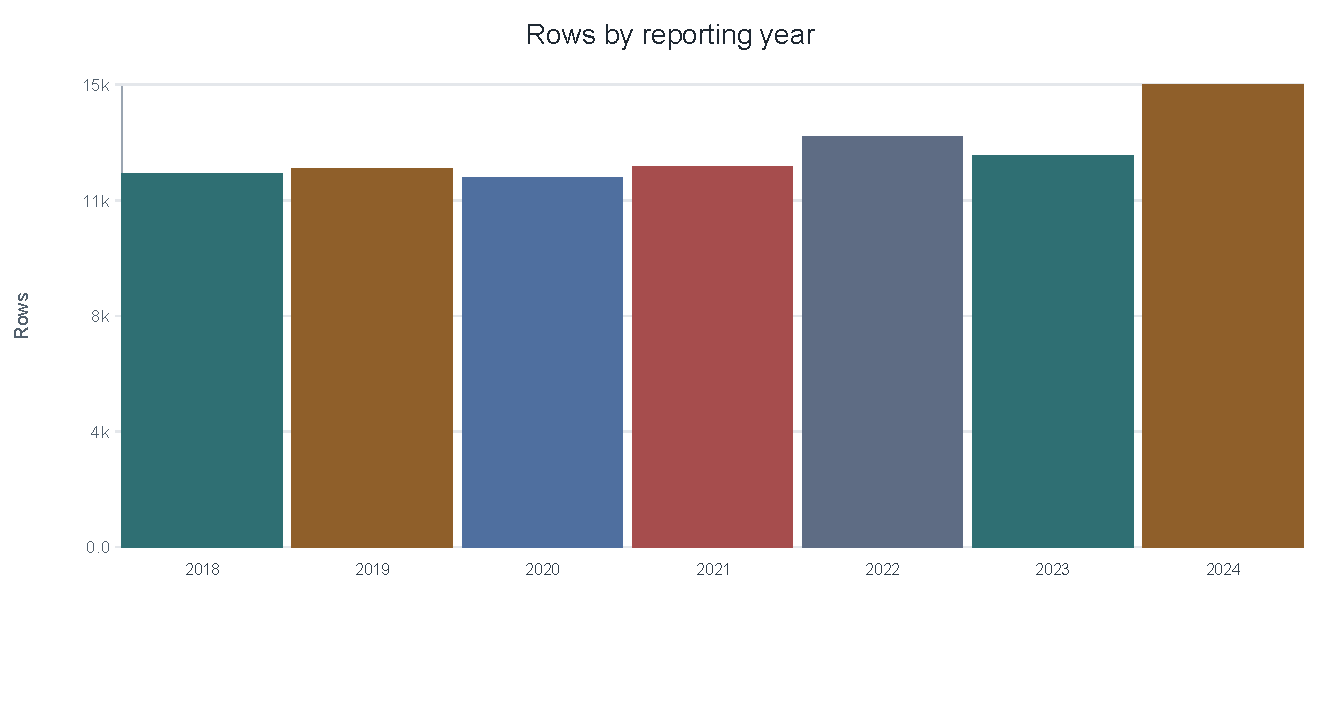
\includegraphics[width=\textwidth]{figures/mrv_rows_by_year.pdf}
\caption{Annual coverage of THETIS-MRV public emission reports from 2018 to 2024.\label{fig:rows}}
\end{figure}

\subsection{Relative Efficiency Label}

The main target is a three-class relative efficiency label derived from the CO2-per-distance variable. Within each \texttt{ship\_type} and \texttt{reporting\_year} group, records are ranked by CO2 emissions per distance and divided into tertiles: \texttt{efficient}, \texttt{medium}, and \texttt{inefficient}. This construction avoids direct comparison of raw CO2 intensity across fundamentally different ship categories and controls for annual shifts in fleet composition and reporting conditions. It also produces approximately balanced classes. The label is descriptive and relative within the MRV dataset; it is not a regulatory compliance label.

\begin{figure}[H]
\centering
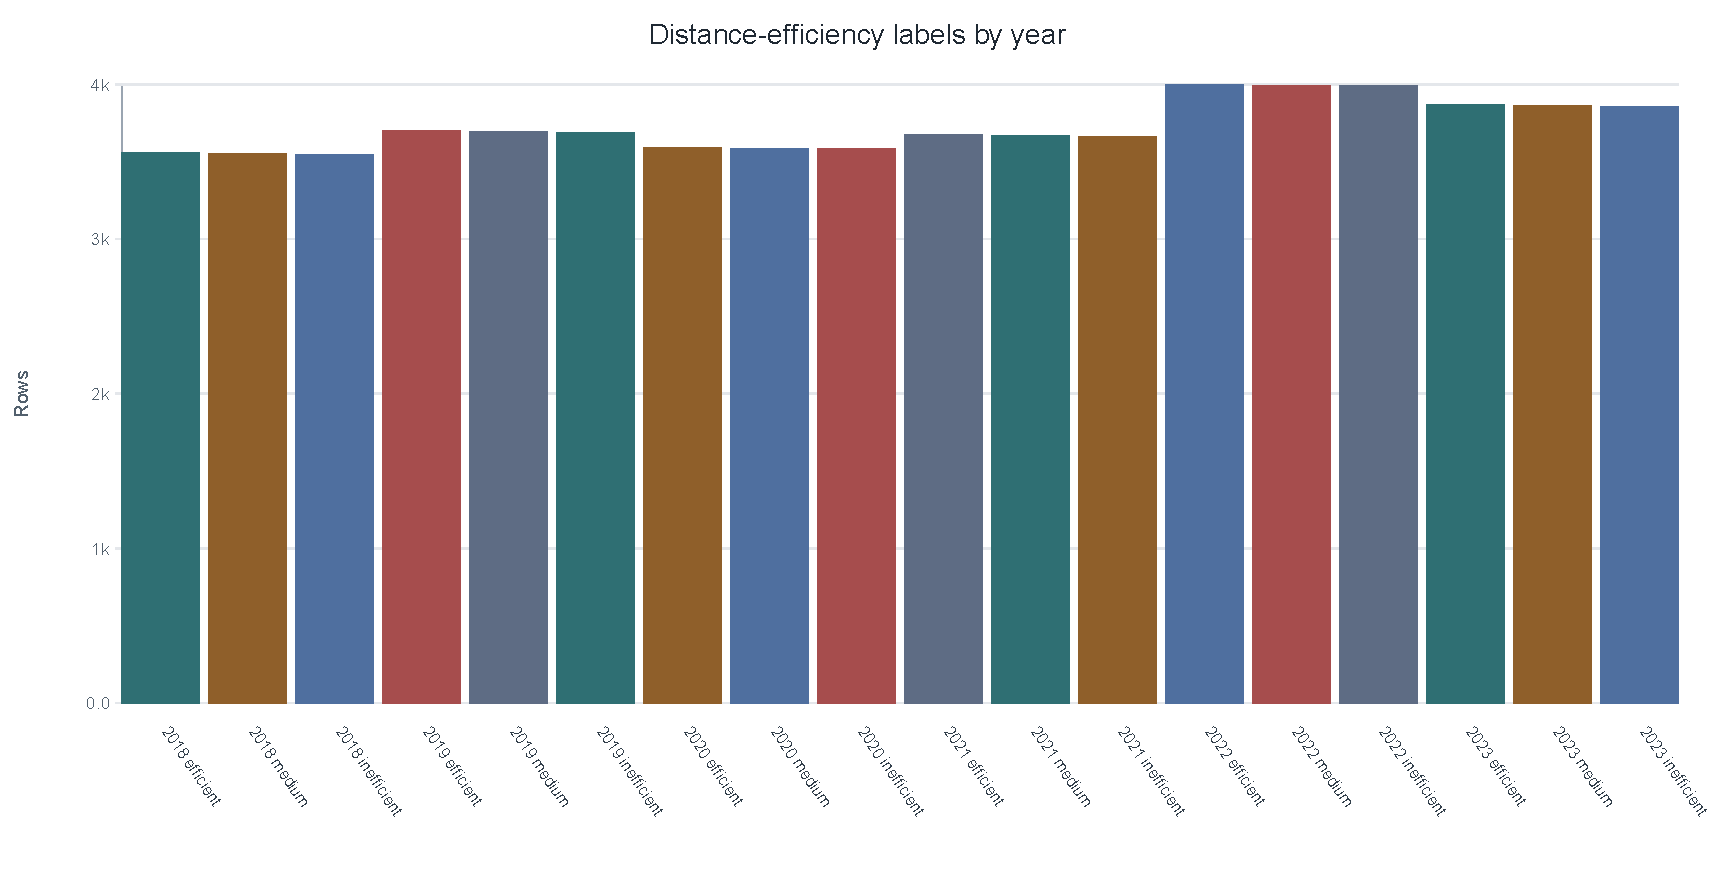
\includegraphics[width=\textwidth]{figures/mrv_label_distribution_by_year.pdf}
\caption{Distribution of ship-type-year tertile labels for CO2 emissions per distance.\label{fig:labels}}
\end{figure}

\subsection{Feature Sets and Leakage Control}

Two non-leakage feature sets are used for the main classification task. The \texttt{strict\_static} set includes reporting year, ship type, parsed technical efficiency fields, port-of-registry information, home-port and ice-class indicators, and monitoring-method indicators. The \texttt{operational\_no\_emission} set adds non-emission operational variables such as time spent at sea and ice-navigation variables.

Target-family fields are excluded from classification. These include CO2 intensity, total CO2 emissions, fuel consumption, fuel intensity, transport-work intensity, and on-laden variants. The broader \texttt{consistency\_screening} field set is reserved for the separate anomaly-screening task.

\subsection{Temporal Evaluation and Models}

The primary evaluation is temporal: models are trained on 2018--2021 labeled records, validated on 2022 records, tested on 2023 records, and checked externally on 2024 full-year labeled records. A random stratified 80/20 split over 2018--2023 is included only as an optimistic comparison. Practical use would require applying a model trained on earlier reports to later reports; therefore, temporal evaluation is the main evidence.

Three classifiers are evaluated: Logistic Regression with class balancing, Random Forest with balanced subsampling, and Histogram-based Gradient Boosting. Numerical features are median-imputed. Categorical features are one-hot encoded for Logistic Regression and Random Forest and ordinal-encoded for Histogram-based Gradient Boosting. Macro-F1 and balanced accuracy are the primary metrics. The implementation uses Python and scikit-learn \cite{scikit_learn}.

\subsection{Ship-Type Ablation, Interpretability, and Consistency Screening}

The ship-type ablation compares a unified model trained on all ship types with separate models trained for the five largest ship types: Bulk carrier, Oil tanker, Container ship, Chemical tanker, and General cargo ship. The ablation uses Histogram-based Gradient Boosting under both non-leakage feature sets.

Permutation importance is computed for the best temporal classifier using Macro-F1 drop after feature permutation. Error analysis focuses on medium-class records, because these records sit near tertile boundaries and are expected to have less stable class membership than the efficient and inefficient extremes.

The consistency-screening module is separate from classification. It uses complete annual reports with positive values for fuel consumption, fuel per distance, total CO2 emissions, CO2 per distance, and time spent at sea. Three methods are used: Isolation Forest, Local Outlier Factor, and regression residual ranking. Candidate rows are described as anomaly-screening candidates for subsequent manual inspection. They are not interpreted as regulatory violations, fraud, or false reporting. Sensitivity is assessed using 1\%, 2\%, and 5\% per-method ship-type thresholds.

\section{Results}

\subsection{Main Temporal Classification}

The best temporal result is obtained by Histogram-based Gradient Boosting with the \texttt{operational\_no\_emission} feature set. On the 2023 test set, it reaches Macro-F1 = 0.603 and balanced accuracy = 0.605. The \texttt{strict\_static} model is close, with Macro-F1 = 0.601 and balanced accuracy = 0.603, indicating that the added non-emission operational fields provide only a small improvement. The random stratified evaluation gives higher performance than the temporal evaluation. The best random split reaches Macro-F1 = 0.657, compared with Macro-F1 = 0.603 in the 2023 temporal test.

\begin{table}[H]
\caption{Classification performance under temporal, external-year, and random stratified evaluation settings.\label{tab:main_results}}
\begin{adjustwidth}{-\extralength}{0cm}
\begin{tabularx}{\fulllength}{LLLLCCC}
\toprule
\textbf{Scenario} & \textbf{Split} & \textbf{Features} & \textbf{Model} & \textbf{Rows} & \textbf{Macro-F1} & \textbf{Balanced Accuracy}\\
\midrule
Temporal & 2023 test & Operational & HGB & 12,615 & 0.603 & 0.605\\
Temporal & 2023 test & Static & HGB & 12,615 & 0.601 & 0.603\\
Temporal & 2023 test & Operational & RF & 12,615 & 0.560 & 0.573\\
Temporal & 2023 test & Static & RF & 12,615 & 0.556 & 0.567\\
External & 2024 full-year & Operational & HGB & 12,905 & 0.585 & 0.587\\
External & 2024 full-year & Static & HGB & 12,905 & 0.580 & 0.582\\
Random & random test & Static & HGB & 14,609 & 0.657 & 0.660\\
Random & random test & Operational & HGB & 14,609 & 0.655 & 0.658\\
\bottomrule
\end{tabularx}
\end{adjustwidth}
\noindent{\footnotesize{HGB = Histogram-based Gradient Boosting; RF = Random Forest; Static = \texttt{strict\_static}; Operational = \texttt{operational\_no\_emission}.}}
\end{table}

\begin{figure}[H]
\centering
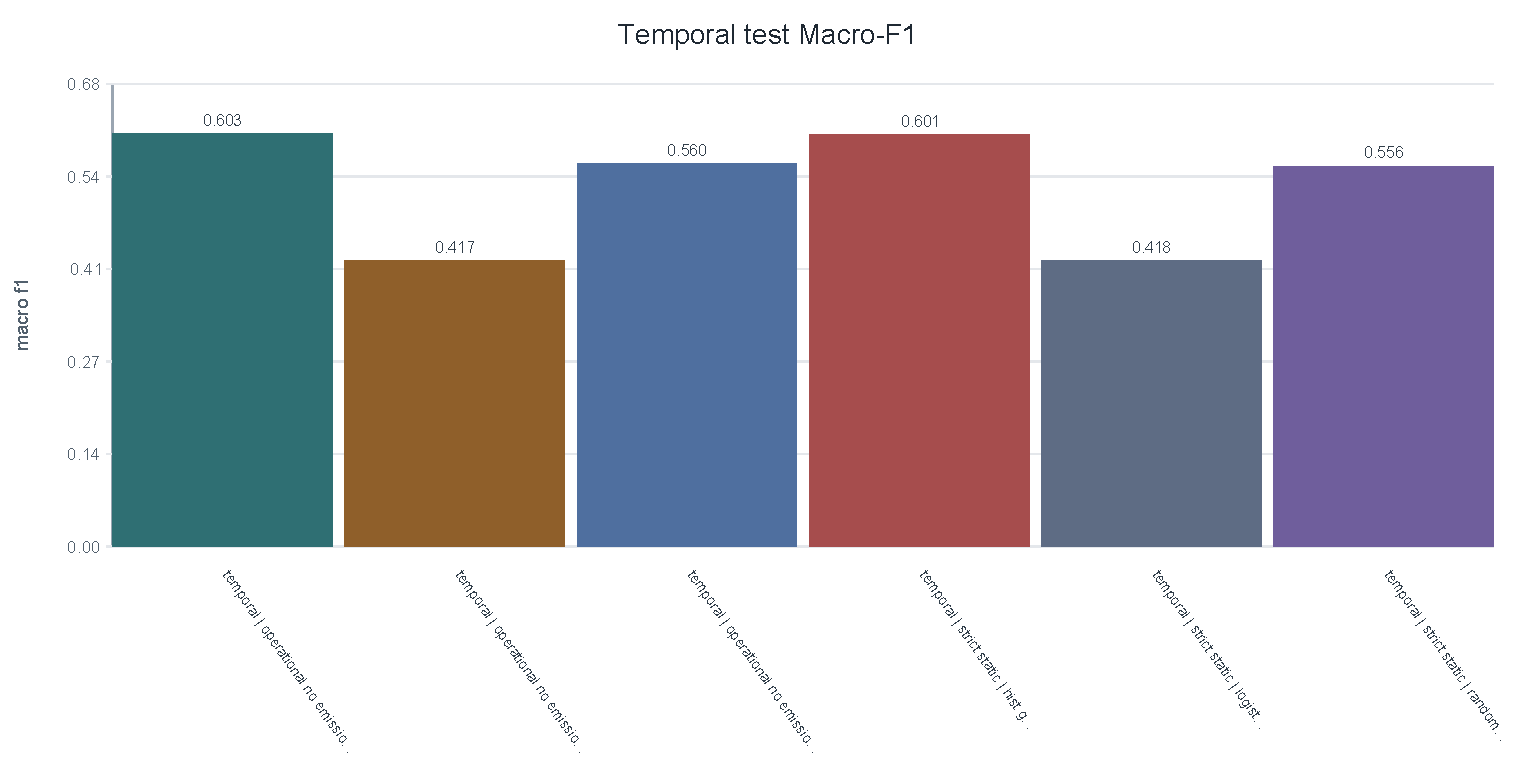
\includegraphics[width=\textwidth]{figures/mrv_baseline_macro_f1_temporal_test.pdf}
\caption{Macro-F1 on the 2023 temporal test set for non-leakage feature sets and baseline classifiers.\label{fig:baseline}}
\end{figure}

\begin{figure}[H]
\centering
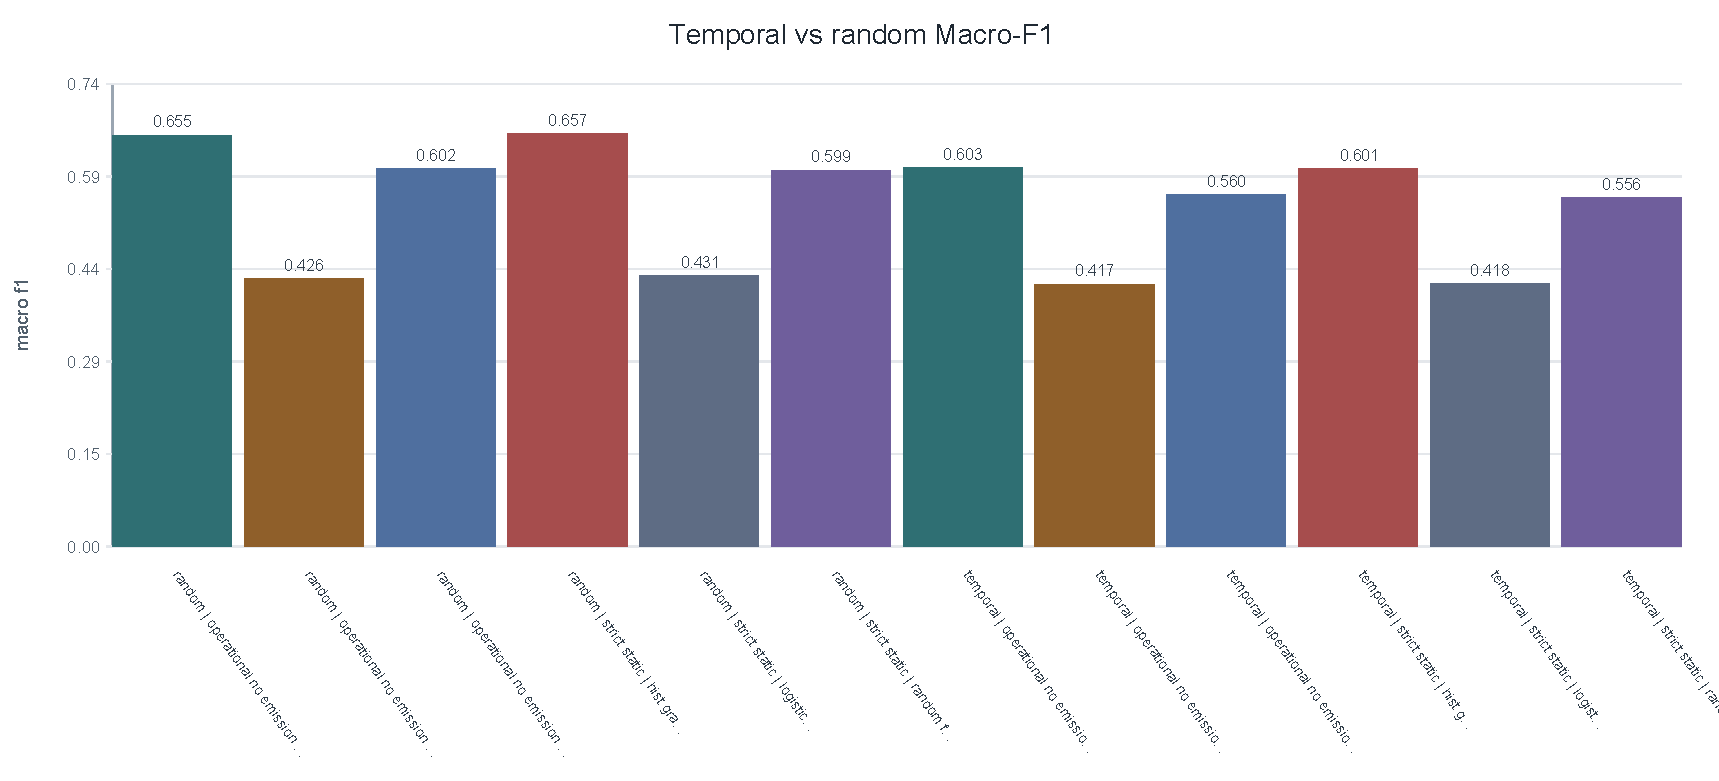
\includegraphics[width=\textwidth]{figures/mrv_random_vs_temporal_macro_f1.pdf}
\caption{Comparison between temporal evaluation and random stratified evaluation.\label{fig:random_vs_temporal}}
\end{figure}

\subsection{Ship-Type Ablation}

Ship-type-specific modeling has heterogeneous effects. General cargo ship benefits under both feature sets, and Container ship improves under \texttt{strict\_static}. Oil tanker shows smaller gains. Bulk carrier does not improve, and Container ship under \texttt{operational\_no\_emission} is slightly worse than the unified model.

\begin{table}[H]
\caption{Unified versus ship-type-specific modeling for the five largest ship categories.\label{tab:ship_type}}
\begin{adjustwidth}{-\extralength}{0cm}
\begin{tabularx}{\fulllength}{LLCCC}
\toprule
\textbf{Ship Type} & \textbf{Features} & \textbf{Unified Macro-F1} & \textbf{Ship-Type Macro-F1} & \textbf{Delta}\\
\midrule
General cargo ship & Static & 0.598 & 0.644 & +0.046\\
Container ship & Static & 0.609 & 0.646 & +0.037\\
General cargo ship & Operational & 0.593 & 0.626 & +0.033\\
Chemical tanker & Operational & 0.566 & 0.583 & +0.017\\
Oil tanker & Static & 0.671 & 0.687 & +0.016\\
Oil tanker & Operational & 0.674 & 0.682 & +0.008\\
Bulk carrier & Operational & 0.590 & 0.588 & -0.003\\
Chemical tanker & Static & 0.571 & 0.568 & -0.003\\
Bulk carrier & Static & 0.583 & 0.579 & -0.004\\
Container ship & Operational & 0.622 & 0.616 & -0.006\\
\bottomrule
\end{tabularx}
\end{adjustwidth}
\noindent{\footnotesize{Static = \texttt{strict\_static}; Operational = \texttt{operational\_no\_emission}.}}
\end{table}

\begin{figure}[H]
\centering
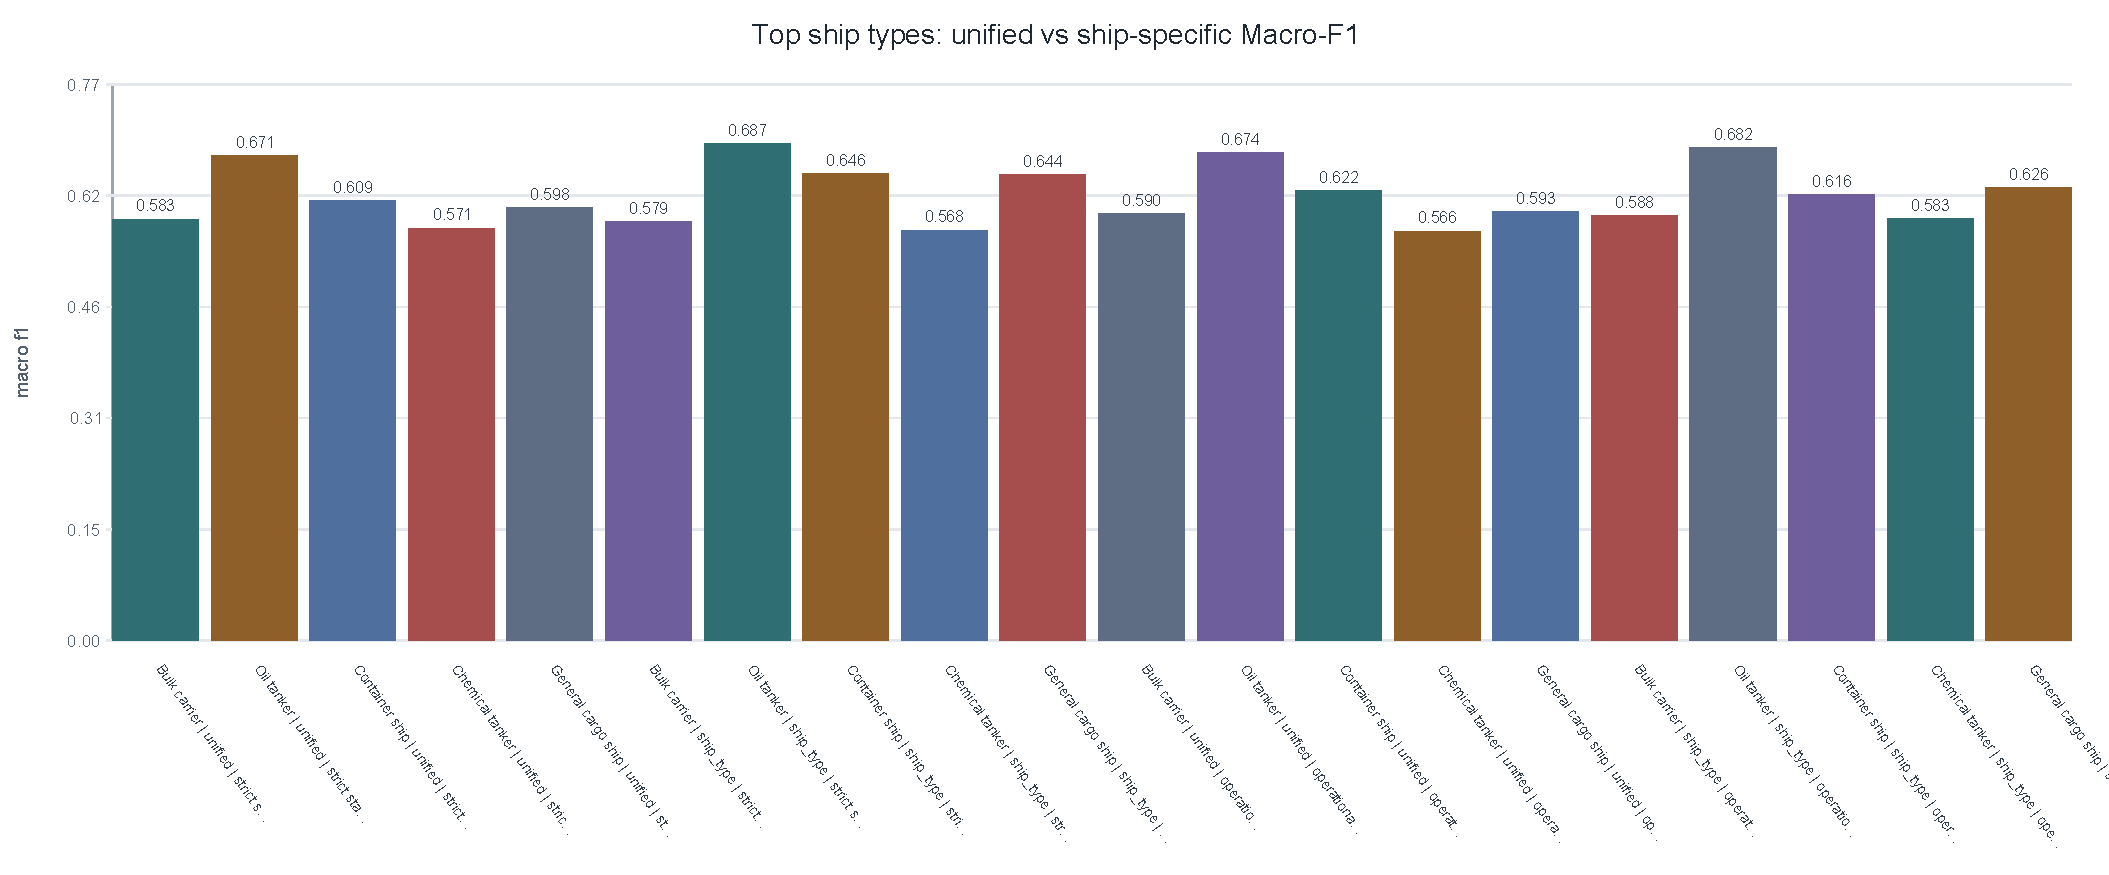
\includegraphics[width=\textwidth]{figures/mrv_ship_type_macro_f1_comparison.pdf}
\caption{Macro-F1 comparison between unified and ship-type-specific models for the five largest ship types.\label{fig:ship_type}}
\end{figure}

\subsection{Feature Importance and Medium-Class Errors}

Permutation importance identifies \texttt{technical\_efficiency\_value} as the strongest non-leakage feature, with a Macro-F1 drop of 0.228 after permutation. The next strongest predictors are \texttt{ship\_type}, \texttt{technical\_efficiency\_type}, \texttt{port\_of\_registry}, and \texttt{time\_spent\_at\_sea\_hours}. The medium class is the main ambiguity source, which is consistent with the tertile-label design.

\begin{table}[H]
\caption{Permutation importance and dominant medium-class error patterns.\label{tab:importance}}
\begin{adjustwidth}{-\extralength}{0cm}
\begin{tabularx}{\fulllength}{LLLC}
\toprule
\textbf{Analysis} & \textbf{Rank} & \textbf{Item} & \textbf{Value}\\
\midrule
Permutation importance & 1 & technical\_efficiency\_value & 0.228\\
Permutation importance & 2 & ship\_type & 0.164\\
Permutation importance & 3 & technical\_efficiency\_type & 0.062\\
Permutation importance & 4 & port\_of\_registry & 0.024\\
Permutation importance & 5 & time\_spent\_at\_sea\_hours & 0.013\\
Medium error & 1 & Bulk carrier medium $\rightarrow$ efficient & 339\\
Medium error & 2 & Container ship medium $\rightarrow$ inefficient & 261\\
Medium error & 3 & General cargo ship medium $\rightarrow$ inefficient & 176\\
Medium error & 4 & Bulk carrier medium $\rightarrow$ inefficient & 169\\
Medium error & 5 & Container ship medium $\rightarrow$ efficient & 161\\
\bottomrule
\end{tabularx}
\end{adjustwidth}
\end{table}

\begin{figure}[H]
\centering
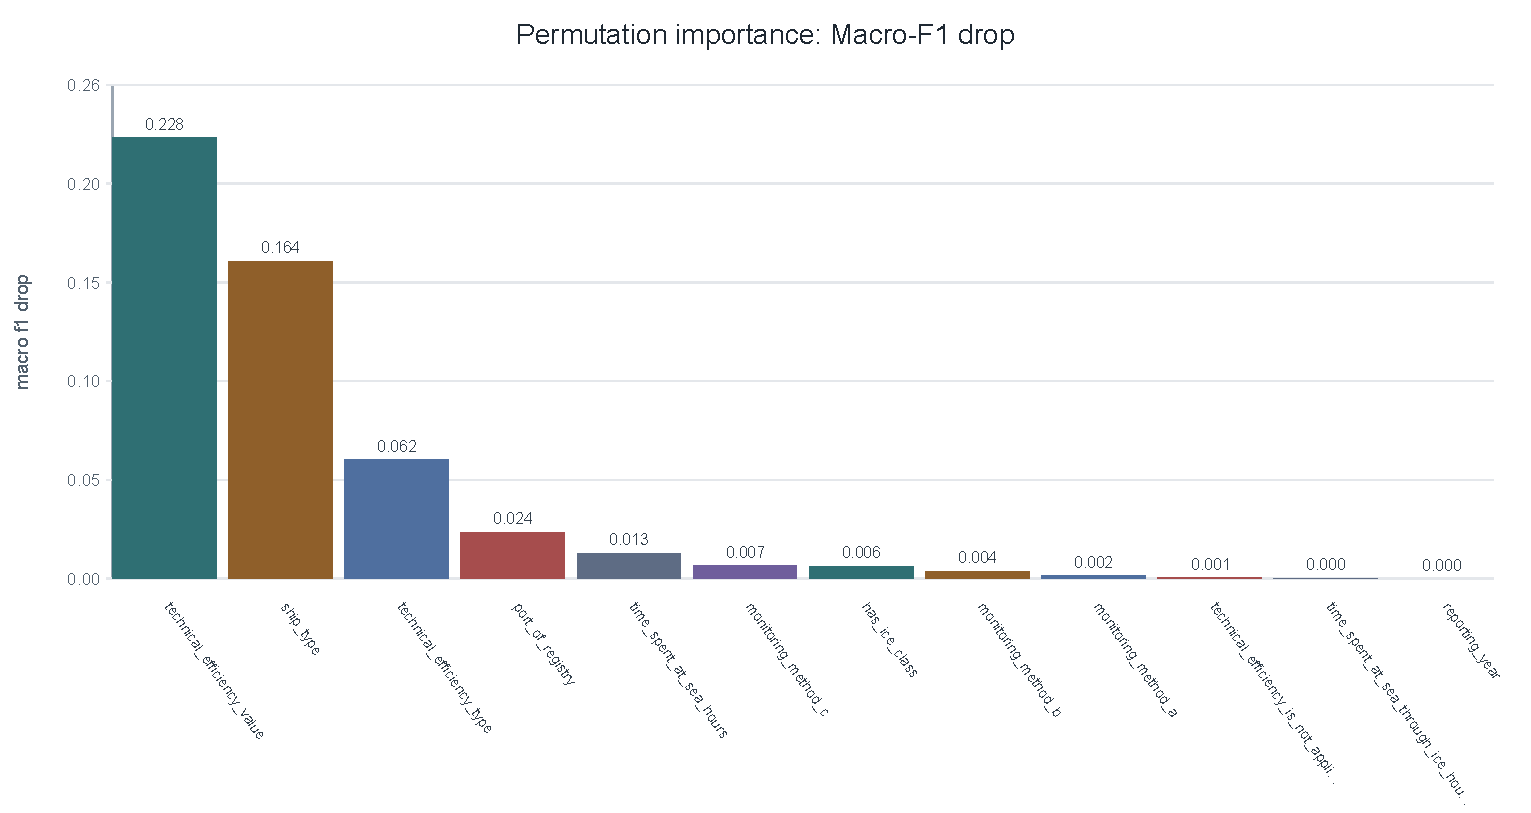
\includegraphics[width=\textwidth]{figures/mrv_permutation_importance_top_features.pdf}
\caption{Permutation importance of the best non-leakage temporal classifier.\label{fig:importance}}
\end{figure}

\subsection{Consistency Screening and Sensitivity Analysis}

The consistency-screening experiment models 85,932 complete annual rows across 14 ship types. At the 2\% threshold, each method flags 1,727 rows. The all-three-method overlap contains 226 rows, while the at-least-two-method set contains 1,067 rows. The top 200 consensus candidates are mainly from Bulk carrier, Oil tanker, General cargo ship, Chemical tanker, and Container ship.

\begin{table}[H]
\caption{Sensitivity of anomaly-screening candidates under 1\%, 2\%, and 5\% ship-type-specific thresholds.\label{tab:sensitivity}}
\begin{adjustwidth}{-\extralength}{0cm}
\begin{tabularx}{\fulllength}{LCCCCCCC}
\toprule
\textbf{Threshold} & \textbf{Isolation} & \textbf{LOF} & \textbf{Residual} & \textbf{All Three} & \textbf{At Least Two} & \textbf{Any Method} & \textbf{Top 200 At Least Two}\\
\midrule
1\% & 865 & 865 & 865 & 97 & 487 & 2,011 & 189\\
2\% & 1,727 & 1,727 & 1,727 & 226 & 1,067 & 3,888 & 200\\
5\% & 4,303 & 4,303 & 4,303 & 643 & 2,626 & 9,640 & 200\\
\bottomrule
\end{tabularx}
\end{adjustwidth}
\end{table}

\begin{figure}[H]
\centering
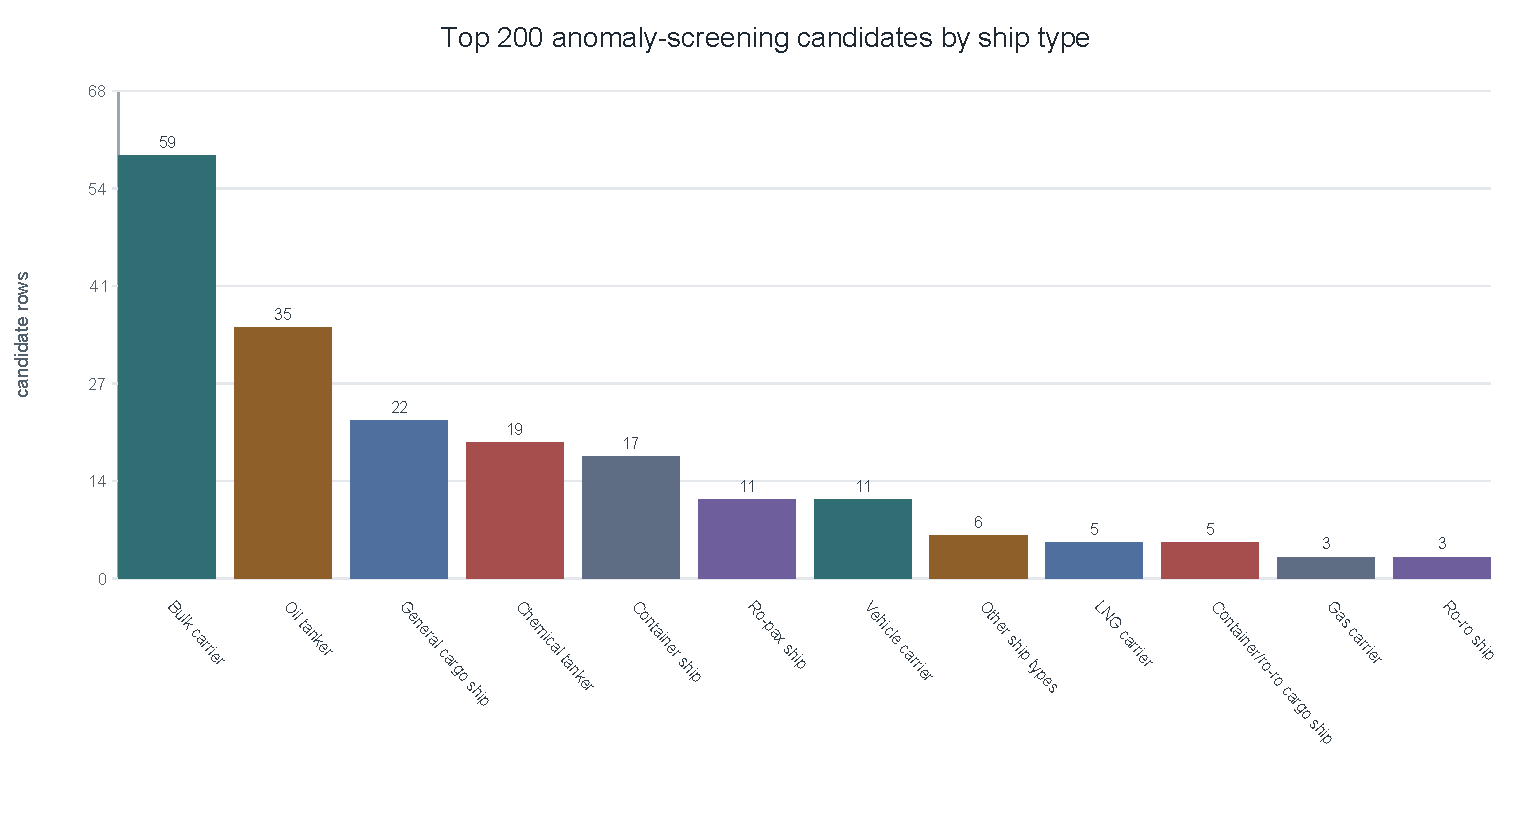
\includegraphics[width=\textwidth]{figures/mrv_anomaly_top_ship_types.pdf}
\caption{Ship-type distribution of the top 200 anomaly-screening candidates.\label{fig:anomaly_ship_types}}
\end{figure}

\begin{figure}[H]
\centering
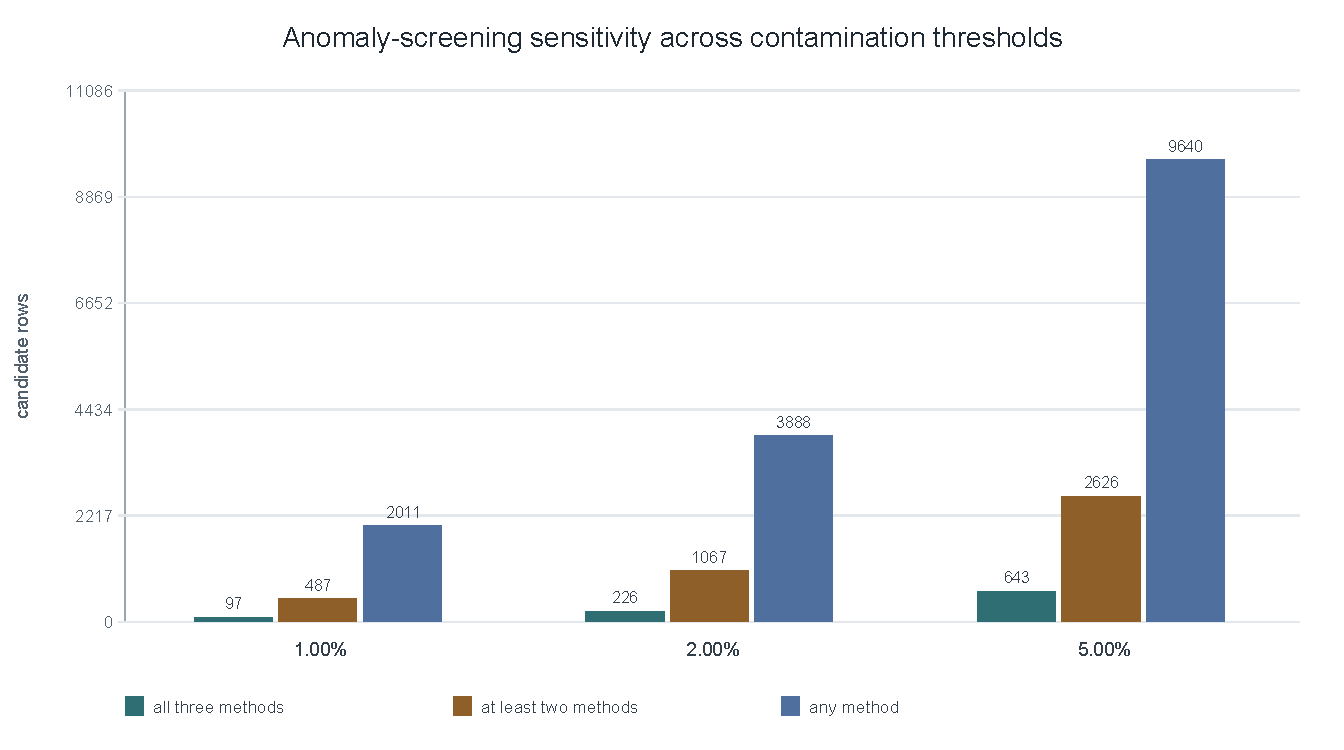
\includegraphics[width=\textwidth]{figures/mrv_anomaly_sensitivity_overlap.pdf}
\caption{Sensitivity of anomaly-screening overlap under 1\%, 2\%, and 5\% thresholds.\label{fig:sensitivity}}
\end{figure}

\section{Discussion}

The results support three main findings. First, public MRV tables contain enough non-leakage information to support moderate temporal prediction of relative ship energy-efficiency strata. The performance level is not high enough to justify automated decision-making, but it is credible for screening, descriptive stratification, and decision-support analysis. The key methodological point is that performance is measured under temporal extrapolation rather than only under a random split.

Second, random stratified evaluation is optimistic for this dataset. A random split can mix similar reporting years and potentially recurring ships across train and test partitions. The observed Macro-F1 gap between the random split and temporal test confirms that annual generalization should be the primary evaluation design for repeated regulatory-reporting datasets.

Third, ship-type specialization is useful only for some categories. This is consistent with the competing effects of fleet heterogeneity and training-sample size. General cargo ship benefits from specialization, whereas Bulk carrier does not. The practical implication is that future applications should not assume a single modeling architecture is best for all ship categories.

The consistency-screening module should be interpreted cautiously. It uses variables that would be leakage-prone in classification, but those same variables are relevant for identifying records with unusual fuel, CO2, distance, time, and intensity combinations. Because no external audit labels are available, the output is a prioritized manual-inspection list rather than proof of incorrect reporting.

Several limitations remain. The tertile label is relative and data-internal; it is not equivalent to CII, EEXI, or any compliance status. The data are annual aggregates and cannot capture voyage-level drivers such as speed, route, weather, loading, or port waiting time. The 2024 schema is broader than earlier schemas, so external-year interpretation requires care. Finally, the current models are deliberately lightweight; future work could compare gradient-boosting libraries specialized for categorical tabular data and could integrate AIS-derived operational variables where licensing permits.

\section{Conclusions}

This study presents MRV-EffScreen, a reproducible framework for public THETIS-MRV ship energy-efficiency stratification and emission consistency screening. Using 2018--2024 public records, the framework constructs ship-type-year relative labels, evaluates non-leakage features under temporal extrapolation, analyzes ship-type heterogeneity, and generates consensus anomaly-screening candidates. The best temporal classifier reaches Macro-F1 = 0.603 on the 2023 test set and Macro-F1 = 0.585 on the 2024 full-year external check, while random stratified evaluation gives a higher and more optimistic estimate. The consistency-screening module identifies stable manual-inspection candidates across threshold settings. The study demonstrates that public MRV data can support transparent machine-learning analysis when leakage control, temporal evaluation, and cautious interpretation are treated as first-order design requirements.

\vspace{6pt}

\authorcontributions{Bo Li is the sole author and completed all CRediT roles: conceptualization, methodology, software, validation, formal analysis, investigation, resources, data curation, writing---original draft preparation, writing---review and editing, visualization, supervision, and project administration. The author has read and agreed to the published version of the manuscript.}

\funding{This research received no external funding.}

\institutionalreview{Not applicable.}

\informedconsent{Not applicable.}

\dataavailability{The original public emission reports are available through the EU THETIS-MRV public emission report portal. The code, processing scripts, metadata, checksums, generated non-sensitive tables, figure files, and manuscript assets are available in the MRV-EffScreen repository at \url{https://github.com/TristanLib/MRV-EffScreen}. A Zenodo DOI will be added if the repository is archived after the first stable release.}

\acknowledgments{The author thanks his family for their support. During the preparation of this manuscript and the associated codebase, AI-assisted tools were used to support drafting, code organization, language editing, and workflow documentation. The author reviewed and edited the outputs and takes full responsibility for the content of this publication.}

\conflictsofinterest{The author declares no conflicts of interest.}

\abbreviations{Abbreviations}{
The following abbreviations are used in this manuscript:
\\

\noindent
\begin{tabular}{@{}ll}
AIS & Automatic Identification System\\
CII & Carbon Intensity Indicator\\
CO2 & Carbon dioxide\\
EEXI & Energy Efficiency Existing Ship Index\\
EU MRV & European Union monitoring, reporting, and verification\\
IMO & International Maritime Organization\\
LOF & Local Outlier Factor\\
MRV & Monitoring, reporting, and verification\\
\end{tabular}
}

\begin{adjustwidth}{-\extralength}{0cm}
\reftitle{References}

\begin{thebibliography}{999}

\bibitem{emsa_thetis_mrv}
European Maritime Safety Agency. THETIS-MRV. Available online: \url{https://emsa.europa.eu/thetis-mrv.html} (accessed on 20 May 2026).

\bibitem{ec_2024_mrv_report}
European Commission, Directorate-General for Climate Action. \textit{2024 Report from the European Commission on CO2 Emissions from Maritime Transport}; 2025. \url{https://doi.org/10.2834/8958061}.

\bibitem{regulation_eu_2015_757}
European Union. Regulation (EU) 2015/757 on the Monitoring, Reporting and Verification of Carbon Dioxide Emissions from Maritime Transport. 2015.

\bibitem{imo_fourth_ghg_study_2020}
International Maritime Organization. \textit{Fourth IMO Greenhouse Gas Study 2020}; 2020.

\bibitem{imo_2023_ghg_strategy}
International Maritime Organization. Revised GHG Reduction Strategy for Global Shipping Adopted. 2023. Available online: \url{https://www.imo.org/en/mediacentre/pressbriefings/pages/revised-ghg-reduction-strategy-for-global-shipping-adopted-.aspx} (accessed on 20 May 2026).

\bibitem{imo_eexi_cii_faq}
International Maritime Organization. EEXI and CII: Ship Carbon Intensity and Rating System. Available online: \url{https://www.imo.org/en/mediacentre/hottopics/pages/eexi-cii-faq.aspx} (accessed on 20 May 2026).

\bibitem{luo2024mrv_review}
Luo, X.; Yan, R.; Wang, S. After Five Years' Application of the European Union Monitoring, Reporting, and Verification (MRV) Mechanism: Review and Prospectives. \textit{J. Clean. Prod.} \textbf{2024}, \textit{434}, 140006. \url{https://doi.org/10.1016/j.jclepro.2023.140006}.

\bibitem{bullock2020shipping_paris}
Bullock, S.; Mason, J.; Broderick, J.; Larkin, A. Shipping and the Paris Climate Agreement: A Focus on Committed Emissions. \textit{BMC Energy} \textbf{2020}, \textit{2}, 5. \url{https://doi.org/10.1186/s42500-020-00015-2}.

\bibitem{liu2008isolation_forest}
Liu, F.T.; Ting, K.M.; Zhou, Z.-H. Isolation Forest. In \textit{Proceedings of the 2008 Eighth IEEE International Conference on Data Mining}; 2008; pp. 413--422. \url{https://doi.org/10.1109/ICDM.2008.17}.

\bibitem{breunig2000lof}
Breunig, M.M.; Kriegel, H.-P.; Ng, R.T.; Sander, J. LOF: Identifying Density-Based Local Outliers. In \textit{Proceedings of the 2000 ACM SIGMOD International Conference on Management of Data}; 2000; pp. 93--104. \url{https://doi.org/10.1145/335191.335388}.

\bibitem{kaufman2012leakage}
Kaufman, S.; Rosset, S.; Perlich, C. Leakage in Data Mining: Formulation, Detection, and Avoidance. \textit{ACM Trans. Knowl. Discov. Data} \textbf{2012}, \textit{6}, 1--21. \url{https://doi.org/10.1145/2382577.2382579}.

\bibitem{scikit_learn}
Pedregosa, F.; Varoquaux, G.; Gramfort, A.; Michel, V.; Thirion, B.; Grisel, O.; Blondel, M.; Prettenhofer, P.; Weiss, R.; Dubourg, V.; VanderPlas, J.; Passos, A.; Cournapeau, D.; Brucher, M.; Perrot, M.; Duchesnay, E. Scikit-learn: Machine Learning in Python. \textit{J. Mach. Learn. Res.} \textbf{2011}, \textit{12}, 2825--2830.

\bibitem{jmse_instructions_2026}
MDPI. Journal of Marine Science and Engineering: Instructions for Authors. Available online: \url{https://www.mdpi.com/journal/jmse/instructions} (accessed on 20 May 2026).

\end{thebibliography}

\PublishersNote{}
\end{adjustwidth}
\end{document}
